\section{Experiments}
In this section, we show the efficacy of the proposed methods using a toy Gaussian model and the MNIST dataset.
\subsection{Projection Method}
In order to prove the rightness of our projection method compared with the traditional projection method in lasso problem, we compared the screening ratio with random generated Gaussian measures by two projection method. We set the $\lambda = \frac{\|\mathbf{X}^{\tranT}y\|}{100}$ and test for 10 different pairs.We choose FISTA for solving $L_2$ penalized UOT problem. 
	\begin{figure}[htbp]
	\begin{center}	
	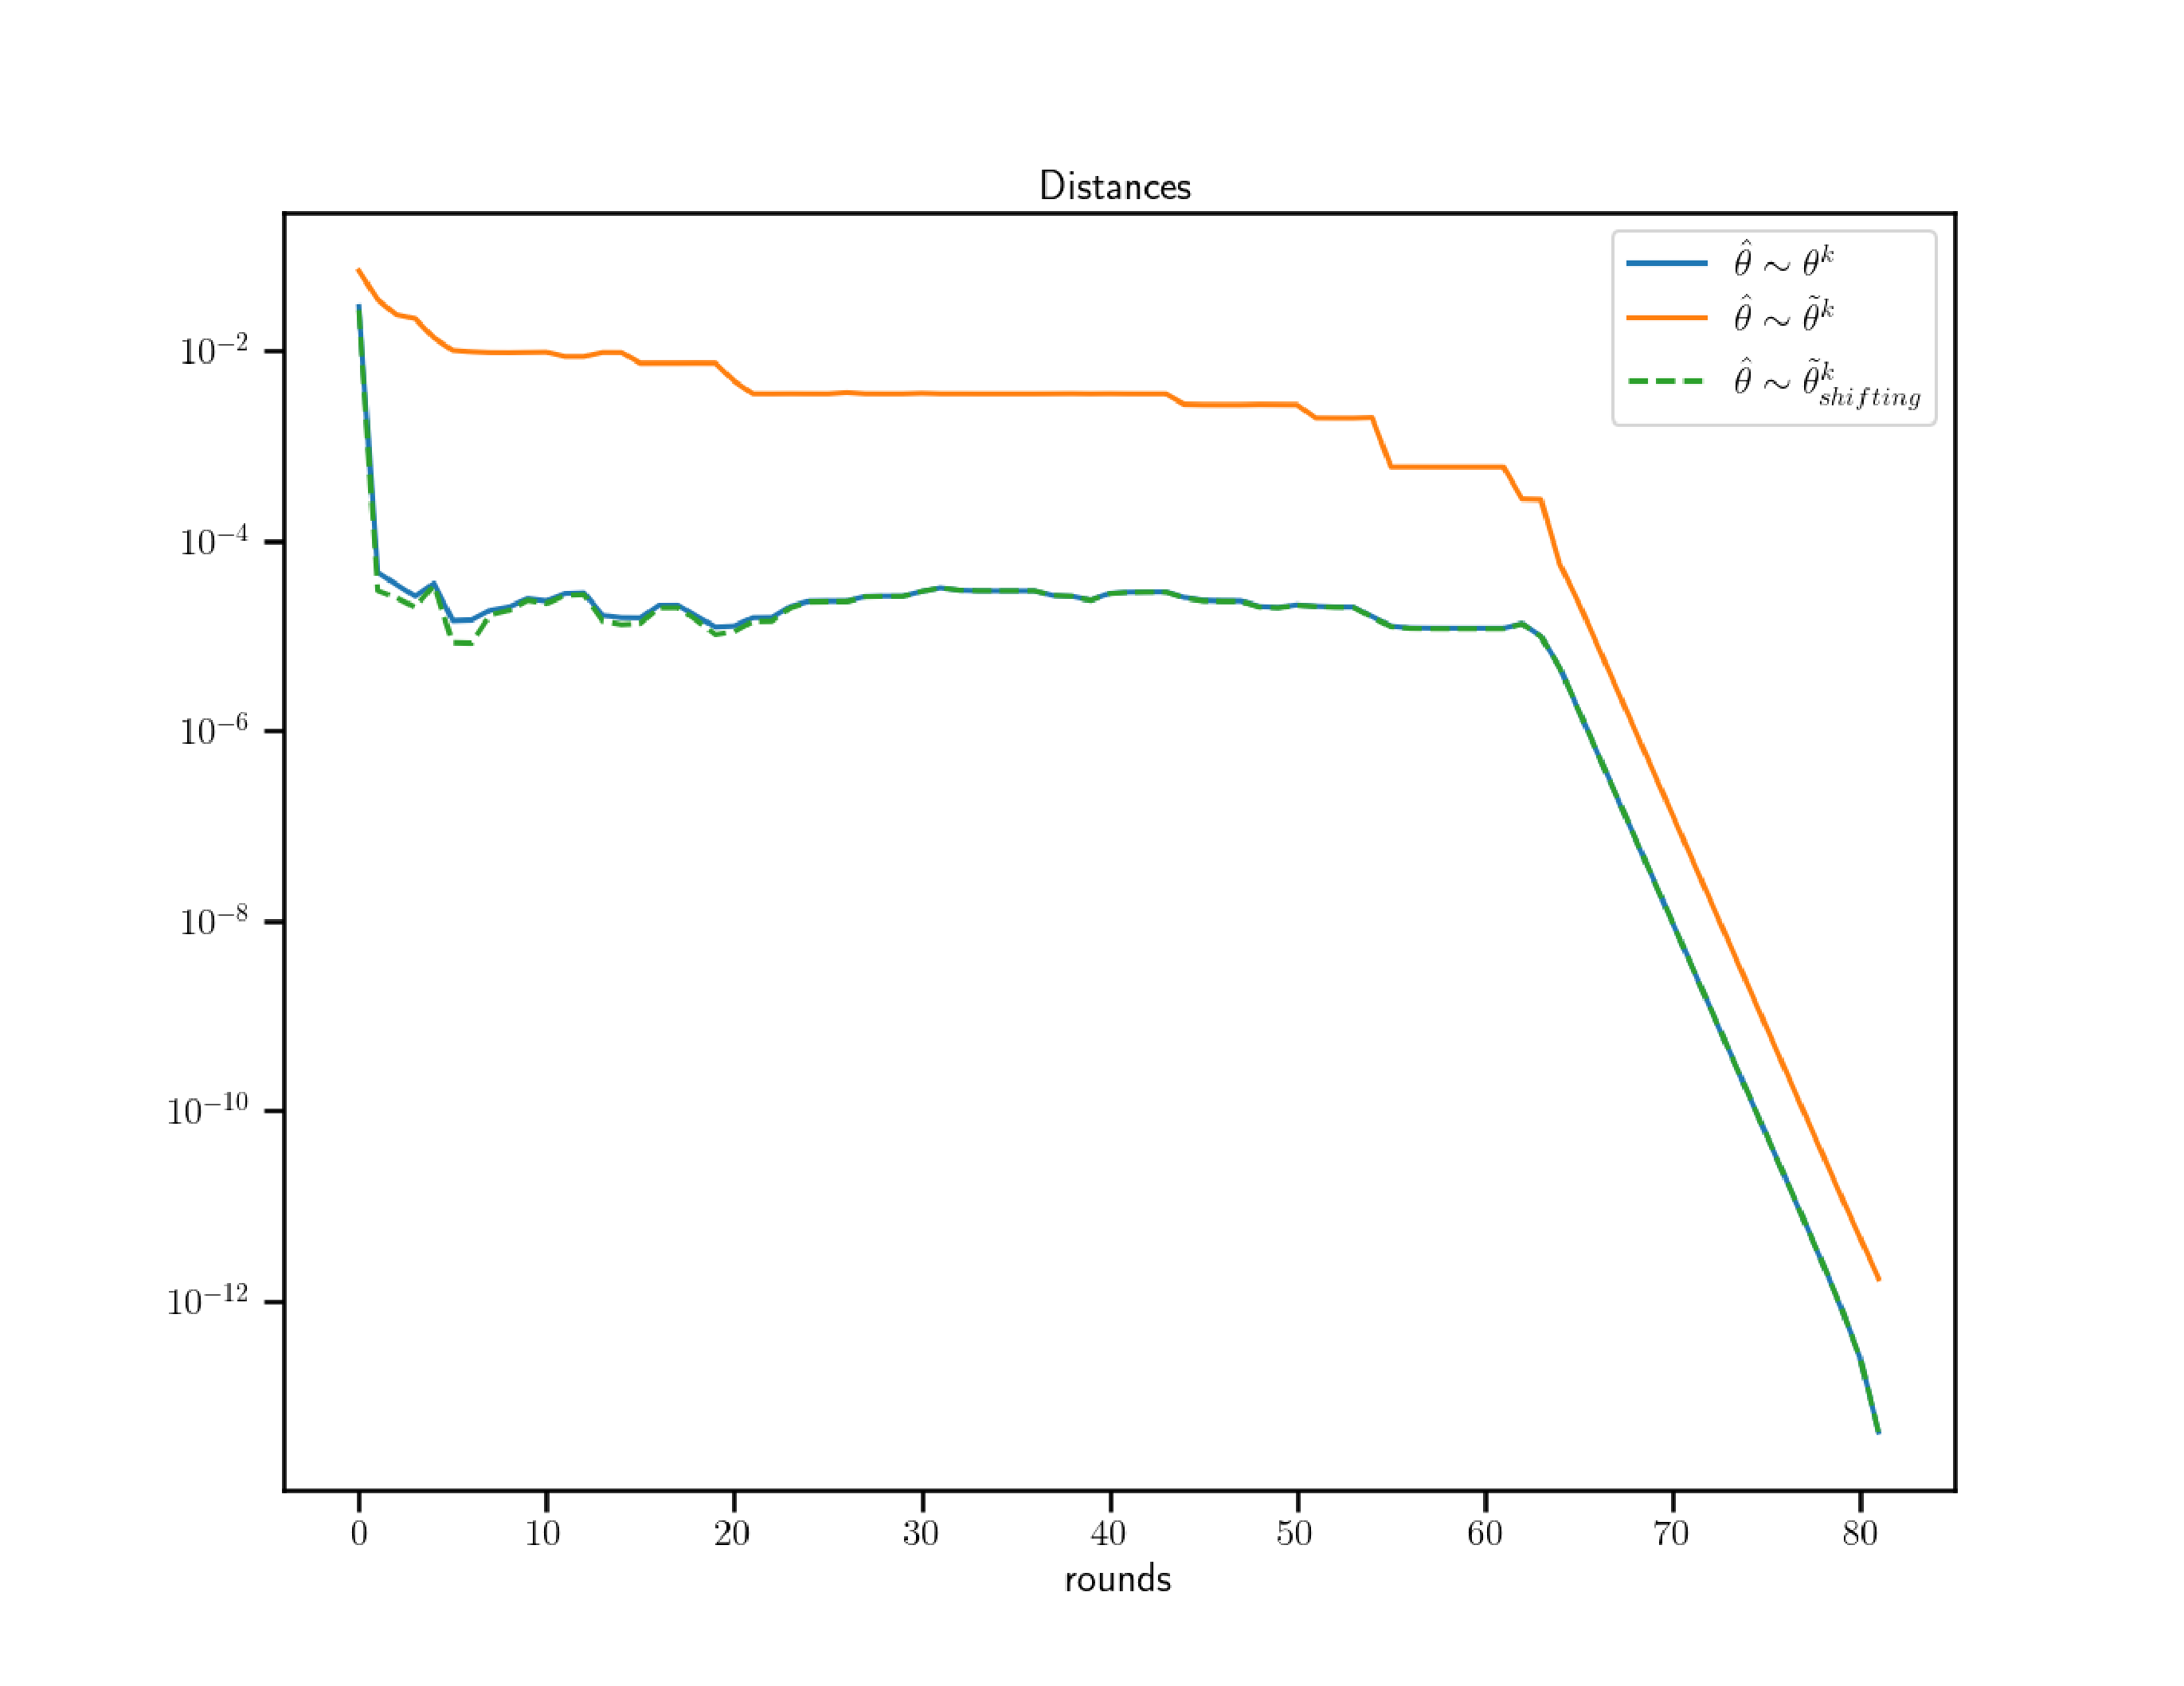
\includegraphics[width=0.4\hsize]{pic/projdis}
	\caption{Distance of different projection method}
	\end{center}	
	\end{figure}
	\begin{figure}[htbp]
	\begin{center}	
	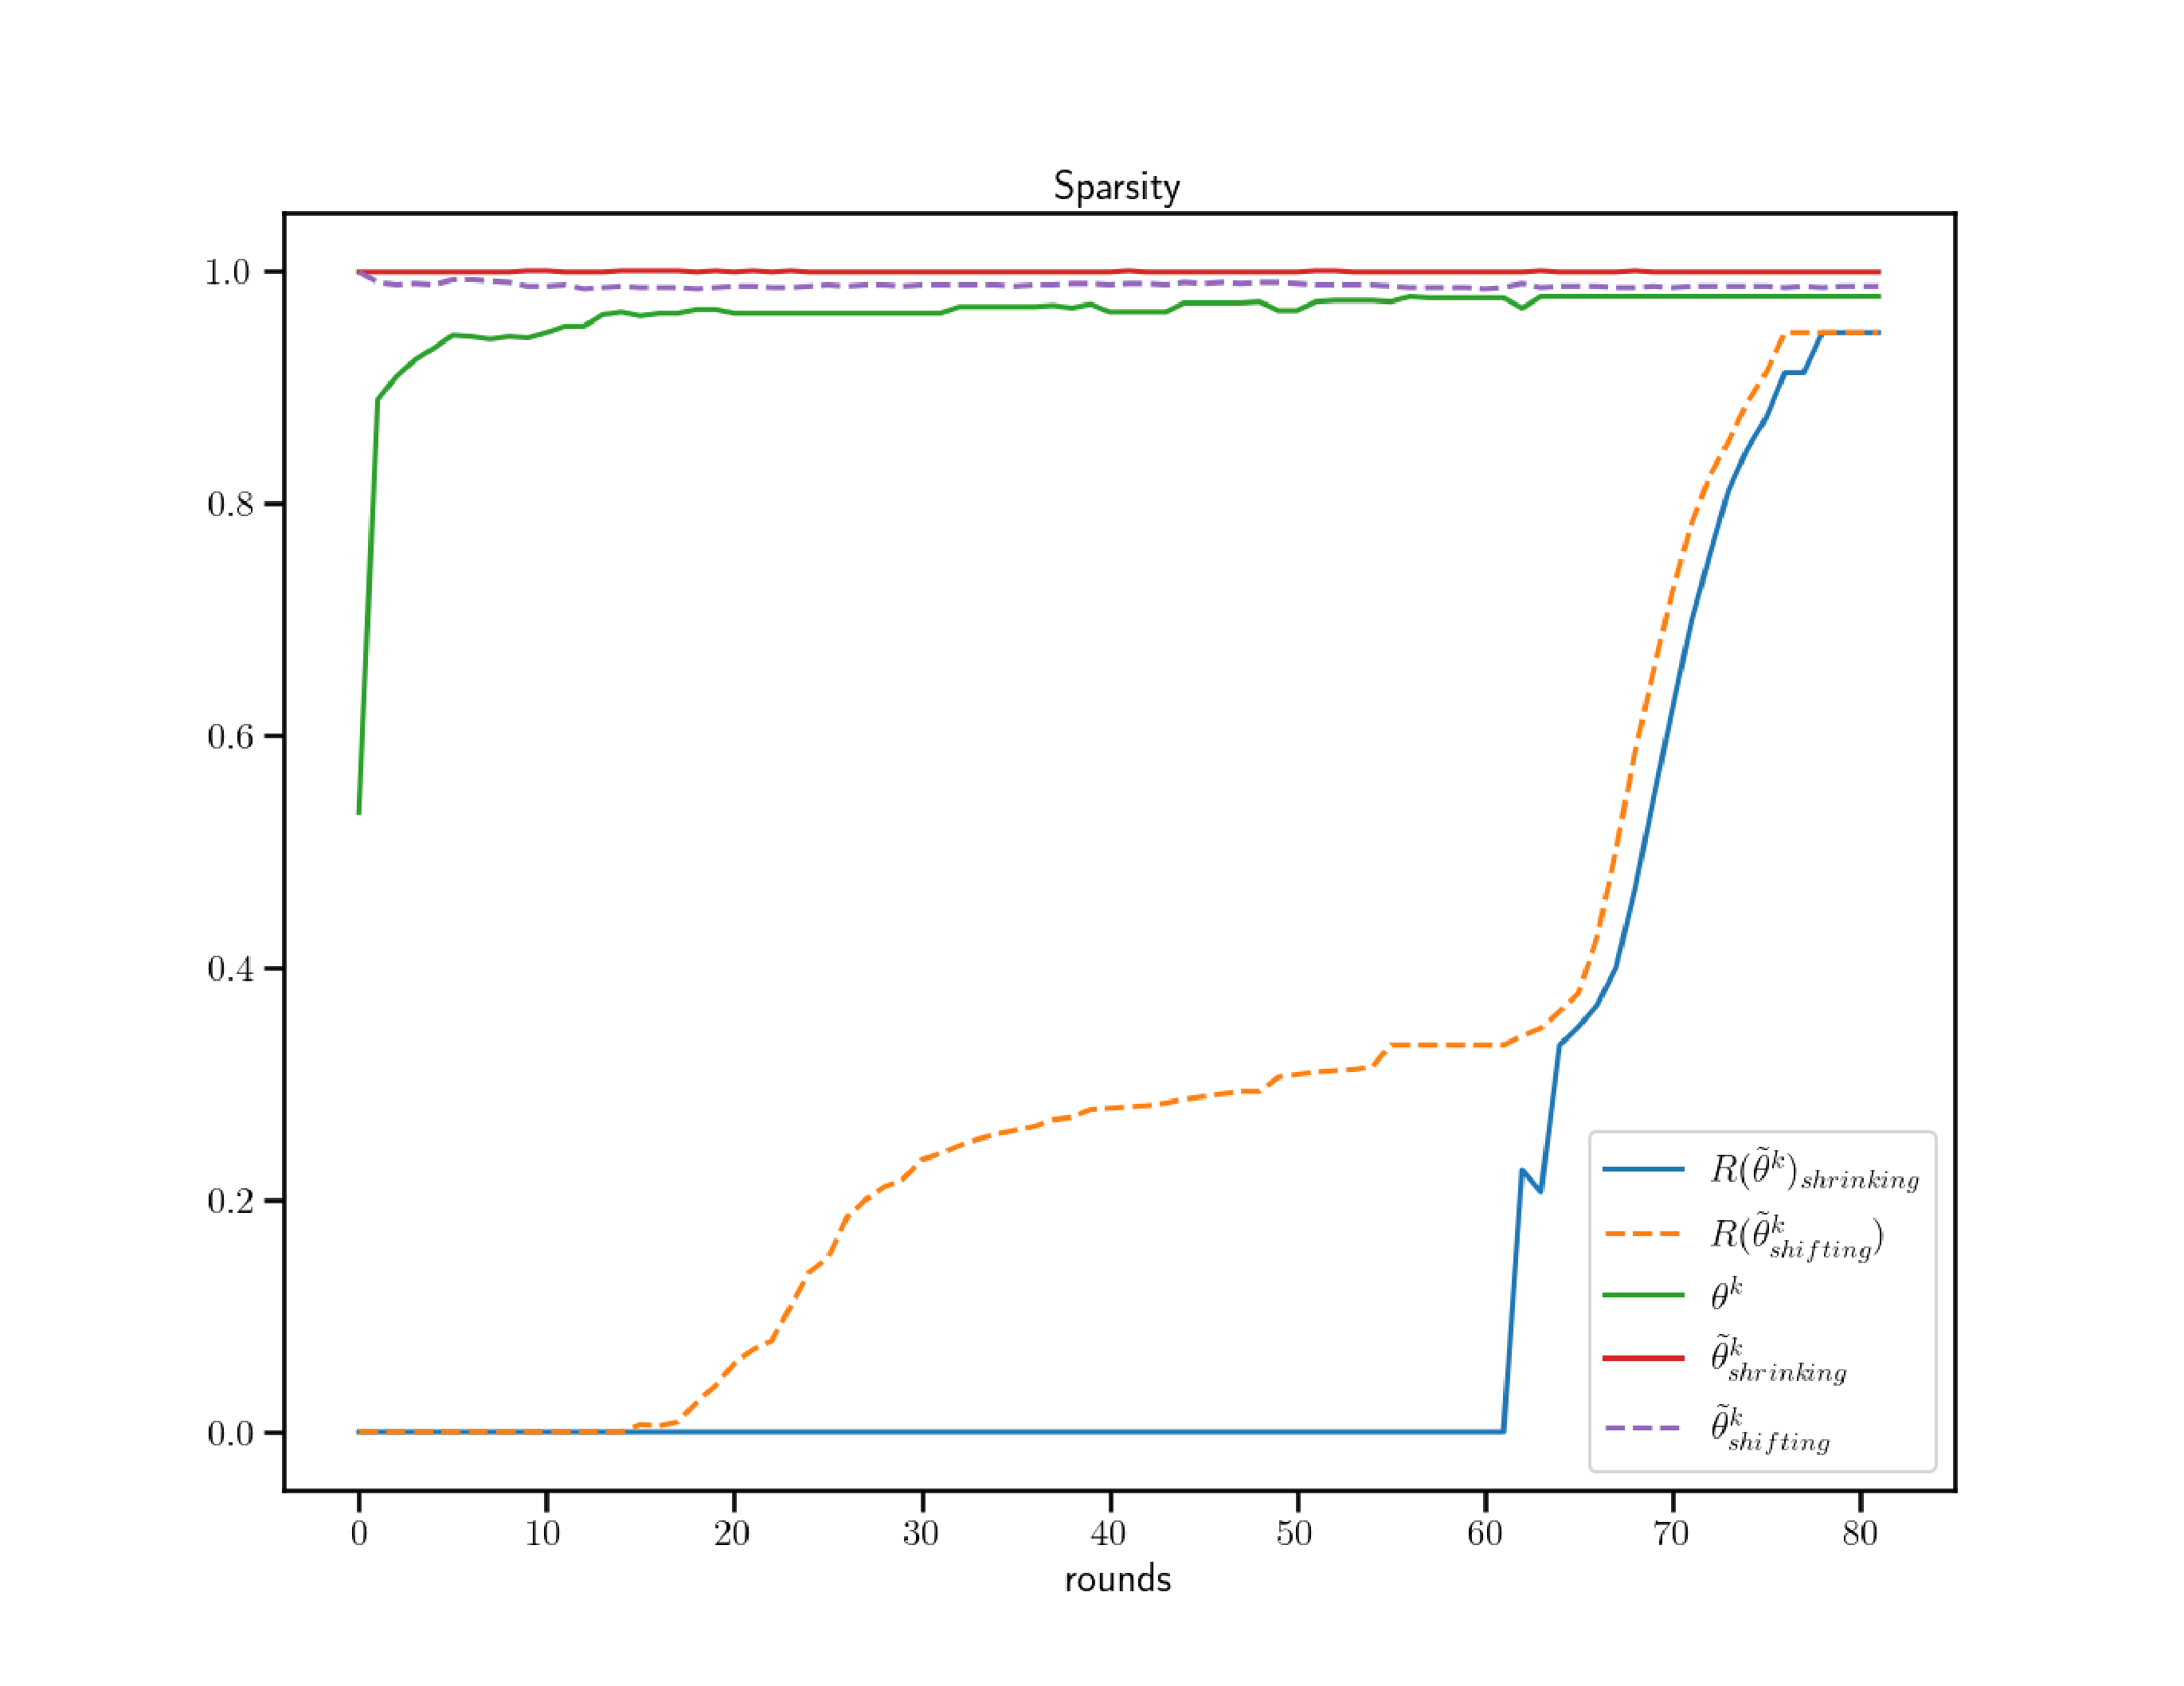
\includegraphics[width=0.4\hsize]{pic/sparse_proj}
	\caption{Screening ratio of different projection method}
	\end{center}	
	\end{figure}

\subsection{Divide Method}
We compared the screening ratio with three different method, including our Divide method, Dynamic Sasvi method and Gap method. 

	\begin{figure}[htbp]
	\begin{center}	
	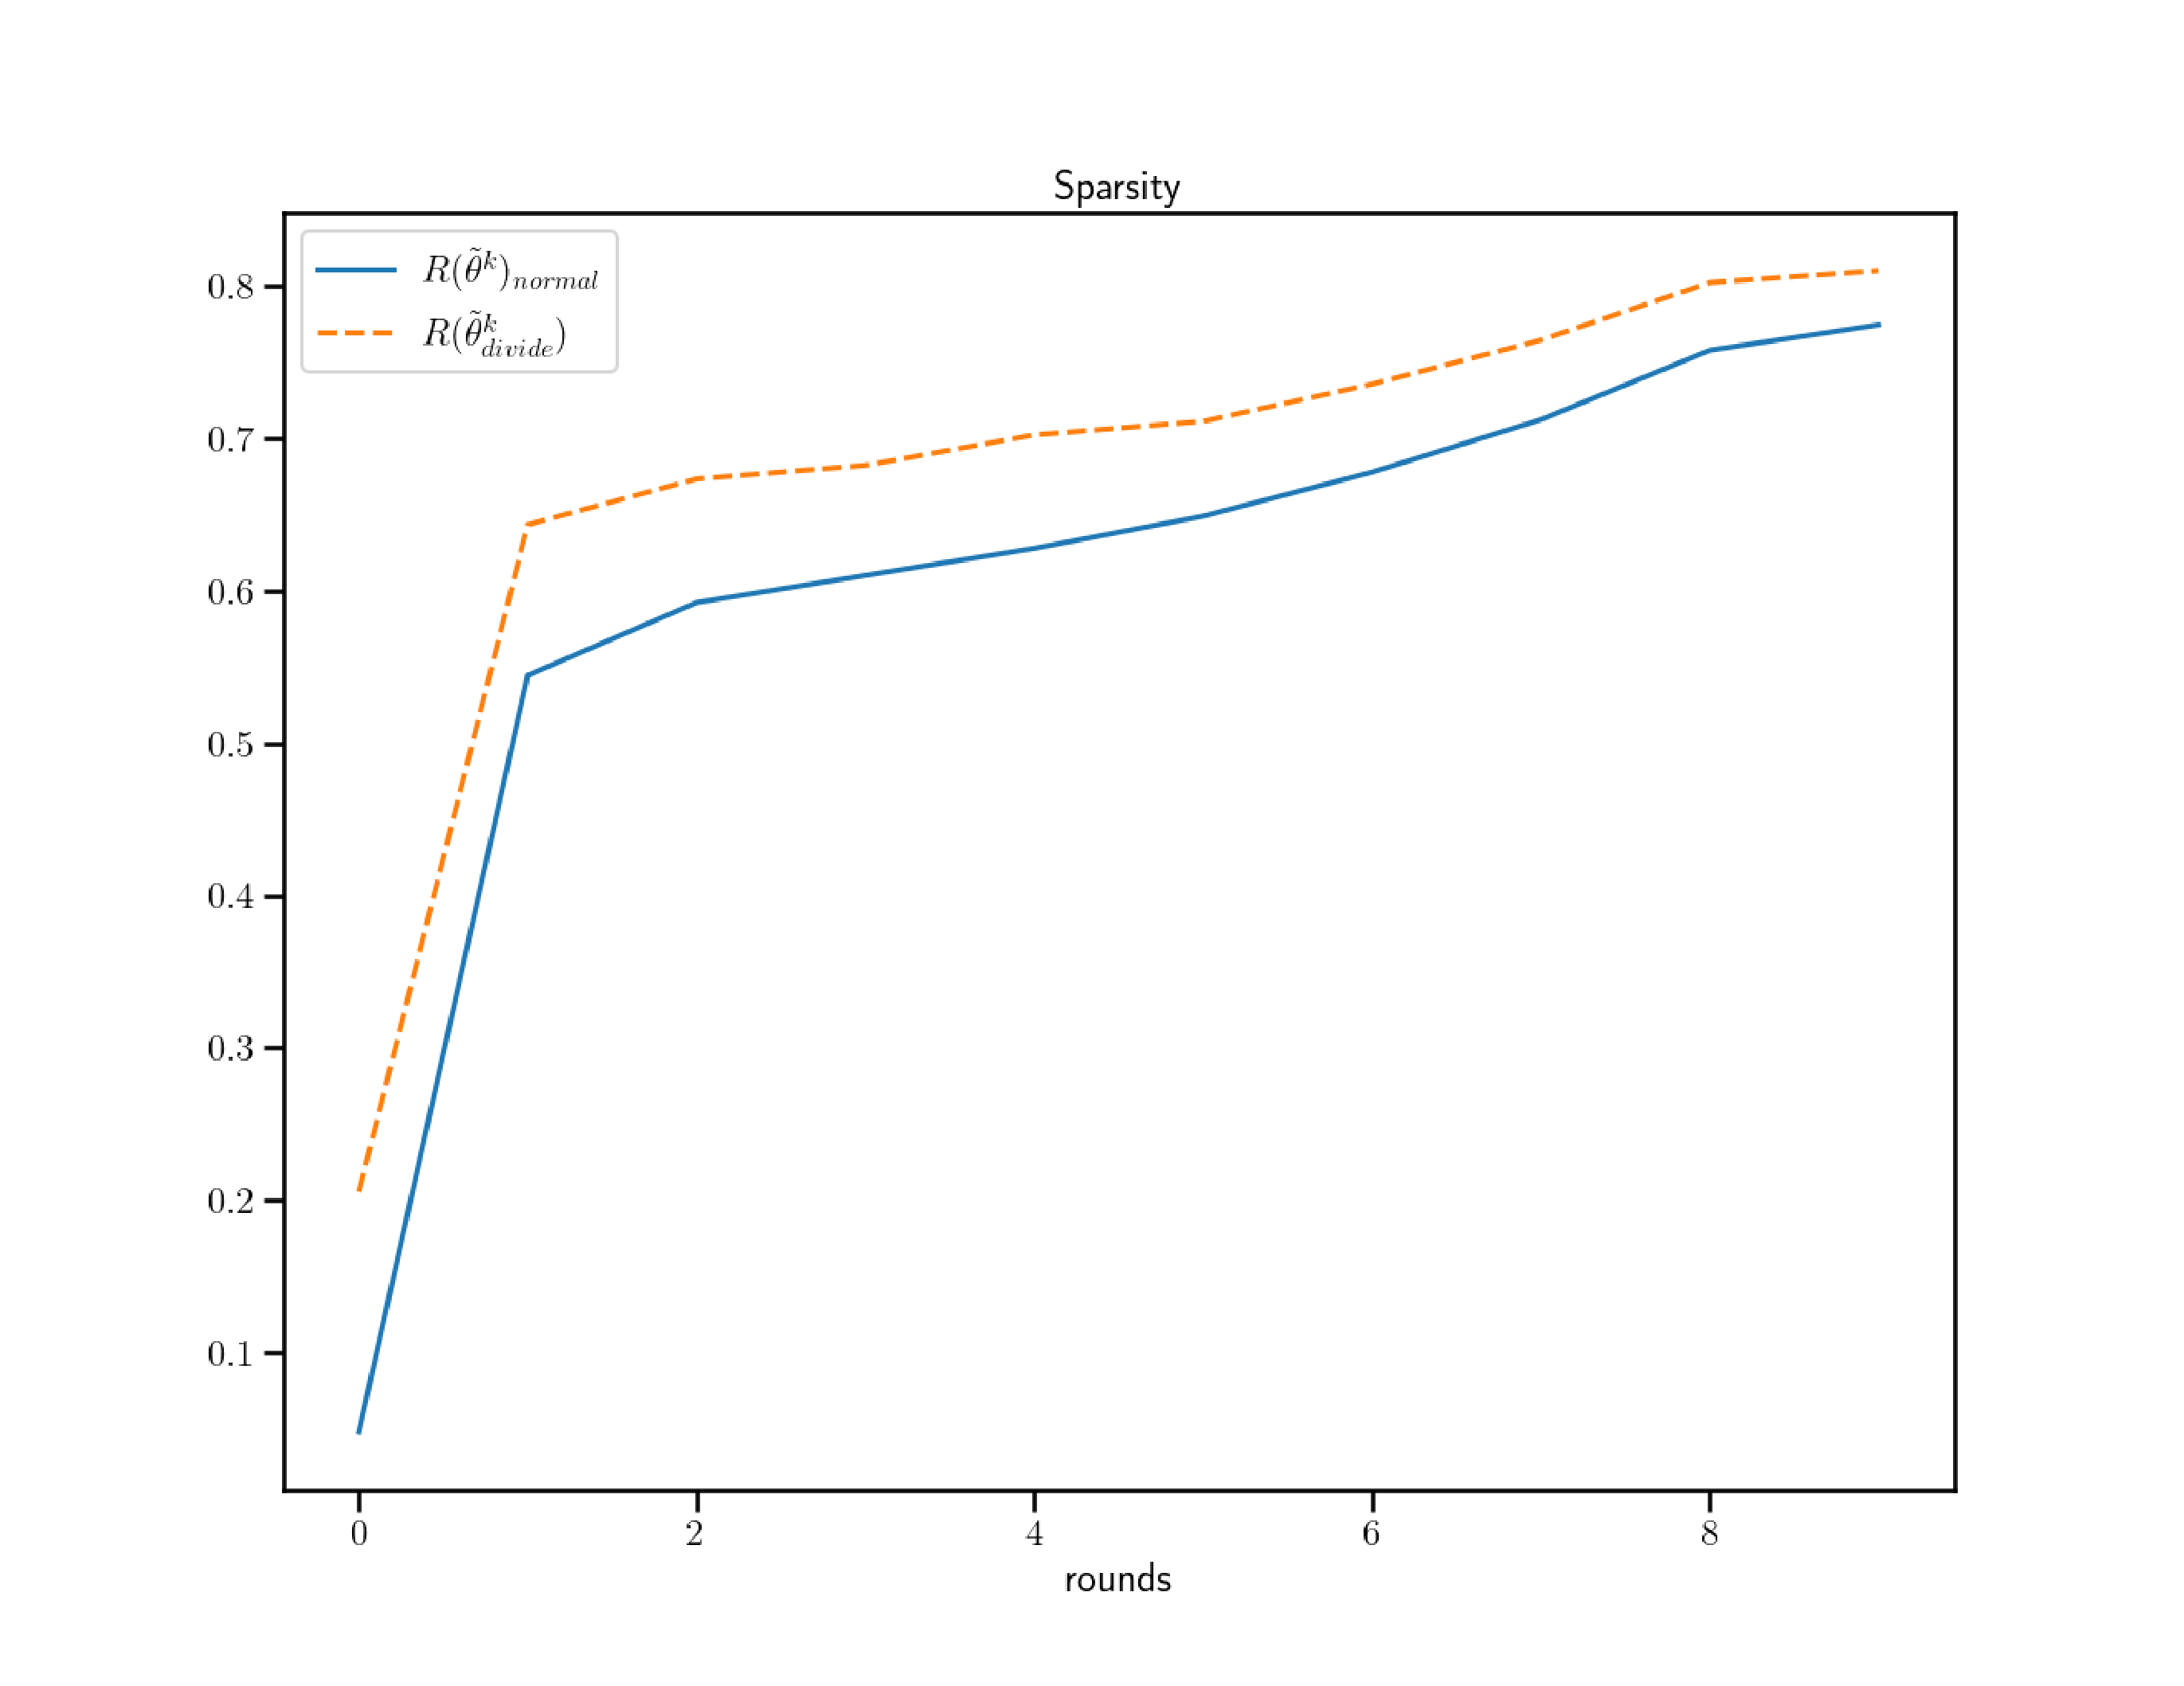
\includegraphics[width=0.4\hsize]{pic/screening_divide_ratio_long}
	\caption{Screening ratio of dividing method}
	\end{center}	
	\end{figure}

\subsection{Best divide Method}
We compared the screening ratio with three different method, including our Divide method, Dynamic Sasvi method and a random divide method.
	\begin{figure}[htbp]
	\begin{center}	
	\includegraphics[width=0.4\hsize]{pic/divide}
	\caption{Comparing of our seperation method with random seperation method}
	\end{center}	
	\end{figure}

\subsection{Speed up ratio}

We choose FISTA method, Newton method and Language method to test about the screening ratio. 
	\begin{figure}[htbp]
	\begin{center}	
	\includegraphics[width=0.4\hsize]{pic/divide}
	\caption{speed up ratio for different solver}
	\end{center}	
	\end{figure}
